\documentclass[runningheads]{llncs}
\usepackage{amsmath}
\usepackage{amsfonts}
\usepackage{mathtools}
\usepackage{color}
\usepackage{graphicx}
\usepackage{listings}
\usepackage{wasysym}
% If you use the hyperref package, please uncomment the following line
% to display URLs in blue roman font according to Springer's eBook style:
% \renewcommand\UrlFont{\color{blue}\rmfamily}

\newcommand\Dist{\mathit{Dist}}
\newcommand\ctrl{\mathit{ctrl}}
\newcommand\prnt{\mathit{prnt}}
\newcommand\link{\mathit{link}}
\newcommand\points{\mathit{points}}
\newcommand\ports{\mathit{ports}}
\newcommand\ar{\mathit{ar}}
\newcommand\id{\mathsf{id}}
\newcommand\Id{\mathsf{Id}}

\providecommand\longrightarrowRHD{\relbar\joinrel\relbar\joinrel\mathrel\RHD}
\providecommand\longrightarrowrhd{\relbar\joinrel\relbar\joinrel\mathrel\rhd}

\makeatletter
\providecommand*\xrightarrowRHD[2][]{\ext@arrow 0055{\arrowfill@\relbar\relbar\longrightarrowRHD}{#1}{#2}}
\providecommand*\xrightarrowrhd[2][]{\ext@arrow 0055{\arrowfill@\relbar\relbar\longrightarrowrhd}{#1}{#2}}
\makeatother

\lstdefinelanguage{Big}{
  sensitive=true,
  morekeywords={fun, brs, end, sbrs, pbrs, nbrs, begin, init, atomic, preds,
    rules, action, big, ctrl, float, int, react},
  comment=[l]{\#}
}

\begin{document}
\title{Nondeterministic Bigraphical Reactive Systems for Markov Decision
  Processes\thanks{Supported by organization x.}}
%\titlerunning{Abbreviated paper title}
% If the paper title is too long for the running head, you can set
% an abbreviated paper title here
\author{Paulius Dilkas\orcidID{0000-1111-2222-3333} \and
  Michele Sevegnani\orcidID{1111-2222-3333-4444}}
\authorrunning{P. Dilkas \& M. Sevegnani}
% First names are abbreviated in the running head.
% If there are more than two authors, 'et al.' is used.
%
\institute{University of Glasgow, Glasgow, UK}
\maketitle

\begin{abstract}
The abstract should briefly summarize the contents of the paper in
150--250 words.

\keywords{First keyword \and Second keyword \and Another keyword.}
\end{abstract}

\section{Introduction}

\begin{definition}[Markov decision process] \label{mdp}
  For any finite set $X$, let $\Dist(X)$ denote the set of discrete probability
  distributions over $X$. A \emph{Markov Decision Process} is a tuple $ (S,
  \overline{s}, A, P, L)$, where: $S$ is a finite set of states and
  $\overline{s} \in S$ is the initial state; $A$ is a finite set of
  \emph{actions}; $P : S \times A \to \Dist(S)$ is a (partial) probabilistic
  transition function, mapping state-action pairs to probability distributions
  over $S$; $L : S \to 2^P$ is a labelling with atomic propositions.
\end{definition}

\begin{definition}[rewards]
  A \emph{reward structure} for an MDP $(S, \overline{s}, A, P, L)$ is a pair
  $(\rho, \iota)$, where $\rho : S \to \mathbb{R}$ is the \emph{state reward
    function}, and $\iota : S \times A \to \mathbb{R}$ is the \emph{transition
    reward function}.
\end{definition}

From \cite{dblp:journals/tcs/sevegnanic15}.

\begin{definition}[concrete place graph with sharing]
  A \emph{concrete place graph with sharing}
  \[ F = (V_F, \ctrl_F, \prnt_F) : m \to n \]
  is a triple having an inner interface $m$ and an outer interface $n$. These
  index the sites and regions of the place graph, respectively. $F$ has a finite
  set $V_F \subset \mathcal{V}$ of nodes, a control map $\ctrl_F : V_F \to
  \mathcal{K}$, and a \emph{parent relation}
  \[ \prnt_F \subseteq (m \uplus V_F) \times (V_F \uplus n) \]
  that is acyclic, i.e., $(v, v) \not\in \prnt_F^+$ for any $v \in V_F$.
\end{definition}

\begin{definition}[composition for place graphs with sharing]
  If $F : k \to m$ and $G : m \to n$ are two concrete place graphs with sharing
  with $V_F \cap V_G = \emptyset$, their composite
  \[ G \circ F = (V, \ctrl, \prnt) : k \to n \]
  has nodes $V = V_F \uplus V_G$ and control map $\ctrl = \ctrl_F \uplus
  \ctrl_G$. Its parent relation $\prnt \subseteq (k \uplus V) \times (V \uplus
  n)$ is given by:
  \[ \prnt \coloneqq \prnt_G^\lhd \uplus \prnt_\circ \uplus \prnt_F^\rhd, \]
  where
  \begin{align*}
    \prnt_F^\rhd &= \prnt_F \rhd V_F, \\
    \prnt_G^\lhd &= V_G \lhd \prnt_G, \\
    \prnt_\circ &= (m \lhd \prnt_G) \circ (\prnt_F \rhd m).
  \end{align*}
\end{definition}

\begin{definition}[tensor product for place graphs]
  If $G_0 : m_0 \to n_0$ and $G_1 : m_1 \to n_1$ are two concrete place graphs
  with sharing with $V_F \cap V_G = \emptyset$, their tensor product
  \[ G_0 \otimes G_1 = (V, \ctrl, \prnt) : m_0 + m_1 \to n_0 + n_1 \]
  has nodes $V = V_{G_0} \uplus V_{G_1}$ and control map $\ctrl \coloneqq
  \ctrl_{G_0} \uplus \ctrl_{G_1}$. Its parent relation $\prnt \subseteq [(m_0 +
  m_1) \uplus V] \times [V \uplus (n_0 + n_1)]$ is defined as
  \[ \prnt_{G_0} \uplus \prnt_{G_1}^{(m_0, n_0)}, \]
  where
  \begin{align*}
    \prnt_{G_1}^{(m_0, n_0)} = &\{ (v, w) \mid (v, w) \in \prnt_{G_1} \text{ and } v, w \in V_{G_1} \} \\
    \uplus &\{ (m_0 + i, w) \mid (i, w) \in \prnt_{G_1}, w \in V_{G_1} \text{ and } i \in m_1 \} \\
    \uplus &\{ (v, n_0 + i) \mid (v, i) \in \prnt_{G_1}, v \in V_{G_1} \text{ and } i \in n_1 \} \\
    \uplus &\{ (m_0 + i, n_0 + j) \mid (i, j) \in \prnt_{G_1}, i \in m_1, \text{ and } j \in n_1 \}.
  \end{align*}
\end{definition}

\begin{definition}[concrete link graph]
  A \emph{concrete link graph}
  \[ F = (V_F, E_F, \ctrl_F, \link_F) : X \to Y \]
  is a quadruple having an inner face $X$ and an outer face $Y$, both finite
  subsets of $\mathcal{X}$, called respectivelly the inner and outer names of
  the link graph. $F$ has finite sets $V_F \subset \mathcal{V}$ of nodes and
  $E_F \subset \mathcal{E}$ of edges, a control map $\ctrl_F : V_F \to
  \mathcal{K}$ and a \emph{link map}
  \[ \link_F : X \uplus P_F \to E_F \uplus Y, \]
  where $P_F \coloneqq \{ (v, i) \mid i \in \ar(\ctrl_F(v)) \}$ is the set of
  ports of $F$. Thus $(v, i)$ is the $i$th port of node $v$. We shall call $X
  \uplus P_F$ the \emph{points} of $F$, and $E_F \uplus Y$ its \emph{links}.
\end{definition}

The sets of points and the set of ports of a link $l$ are defined by
\[ \points_F(l) \coloneqq \{ p \mid \link_F(p) = l \}, \quad \ports_F(l)
  \coloneqq \points_F(l) \setminus X. \]
An edge is \emph{idle} if it has no points. Identities over name sets are
defined by $\id_X = (\emptyset, \emptyset, \emptyset, \Id_X) : X \to X$.

\begin{definition}[concrete bigraph with sharing]
  A concrete bigraph
  \[ F = (V_F, E_F, \ctrl_F, \prnt_F, \link_F) : \langle k, X \rangle \to
    \langle m, Y \rangle \]
  consists of a concrete place graph with sharing $F^P = (V_F, \ctrl_F, \prnt_F)
  : k \to m$ and a concrete link graph $F^L = (V_F, E_F, \ctrl_F, \link_F) : X
  \to Y$. If $X = \epsilon$, then $F$ is called \emph{ground}. We write the
  concrete bigraph with sharing as $F = (F^P, F^L)$.
\end{definition}

Definitions: support translation, lean-support equivalence, concretion,
abstraction.

More definitions: level, normalised levels, occurrence, matching, concrete
occurrence, underlying graph

Stochastic bigraphs \cite{DBLP:journals/entcs/KrivineMT08}

From PhD thesis \cite{DBLP:phd/ethos/Sevegnani12}

% TODO: not general enough
\begin{definition}[reaction rule] \label{reaction_rule}
  A \emph{reaction rule} is a pair
  \[ \mathsf{R} = (R : m \to J, R' : m \to J), \]
  sometimes written as $R \longrightarrowRHD R'$, where $R$ is the \emph{redex}
  and $R'$ the \emph{reactum}, and $R$ is solid. The rule generates all the
  \emph{ground reaction rules} $(r, r')$, where $r = (R \otimes \id_Y) \circ d$
  and $r' = (R' \otimes \id_Y) \circ d$ for some discrete ground
  \emph{parameter} $d : \epsilon \to \langle m, Y \rangle$. The \emph{reaction
    relation} $\longrightarrowrhd_{\mathsf{R}}$ over ground bigraphs is defined
  by
  \[ g \longrightarrowrhd_{\mathsf{R}} g' \text{ iff } g = Dr \text{ and } g' = Dr' \]
  for some bigraph $D$ and some ground reaction rule $(r, r')$ generated from
  $\mathsf{R}$.
\end{definition}

\begin{definition}[bigraphical reactive system (BRS)]
  A \emph{bigraphical reactive system} consists of a pair $(\mathcal{B},
  \mathcal{R})$, where $\mathcal{B}$ is a set of agents and $\mathcal{R}$ is a
  set of reaction rules defined over $\mathcal{B}$. It has a reaction relation
  \[ \longrightarrowrhd_{\mathcal{R}} \coloneqq \bigcup_{\mathsf{R} \in
      \mathcal{R}} \longrightarrowrhd_{\mathsf{R}}, \]
  which will be written $\longrightarrowrhd$ when $\mathcal{R}$ is understood.
\end{definition}

\subsection{Probabilistic bigraphs}

\begin{definition}[probabilistic reaction rule]
  A \emph{probabilistic reaction rule} $\mathsf{R}$ is a triple $(R, R', p)$,
  sometimes written $R \xrightarrowRHD{p} R'$, where $(R, R')$ is a reaction
  rule and $p \in (0, 1]$ is a probability. Similarly to
  Definition~\ref{reaction_rule}, it generates a set of ground reaction rules of
  the form $(r, r', p)$.
\end{definition}

\begin{definition}[probabilistic bigraphical reactive system (PBRS)]
  A \emph{probabilistic bigraphical reactive system} consists of a pair
  $(\mathcal{B}, \mathcal{R})$, where $\mathcal{B}$ is a set of agents and
  $\mathcal{R}$ is a set of probabilistic reaction rules defined over
  $\mathcal{B}$.

  Let $g, g'$ be ground bigraphs, and $\{ (r_i, r'_i, p_i) \}_{i=1}^n$ a set of
  ground probabilistic reaction rules, where for each $r_i$, there exists a
  bigraph $D_i$ such that $g = D_ir_i$. Let $S = \{ (r_i, r'_i, p_i) \mid g' =
  D_ir'_i \}$ (for the same $D_i$), and
  \[ s = \sum_{i=1}^n p_i. \]
  Then the reaction relation is defined as
  \[ g \xrightarrowrhd{p}_{\mathcal{R}} g' \text{ iff } S \ne \emptyset, \]
  where
  \[ p = \frac{1}{s}\sum_{(r, r', p') \in S} p'. \]
\end{definition}

\subsection{Nondeterministic bigraphs}

\begin{definition}[nondeterministic reaction rule]
  Let $A$ be a set of actions. A \emph{nondeterministic reaction rule}
  $\mathsf{R}$ is a tuple $(R, R', a, p)$, where $(R, R', p)$ is a probabilistic
  reaction rule, and $a \in A$ is an action. We also define a \emph{reaction
    reward function} $r : A \to \mathbb{R}$ that assigns a reward/cost to each
  action.
\end{definition}

\begin{definition}[nondeterministic bigraphical reactive system (NBRS)]
  A \emph{nondeterministic bigraphical reactive system} consists of a pair
  $(\mathcal{B}, \mathcal{R})$, where $\mathcal{B}$ is a set of agents and
  $\mathcal{R}$ is a set of nondeterministic reaction rules defined over
  $\mathcal{B}$.

  Let $g, g'$ be ground bigraphs, $a \in A$ an action, and $\{ (r_i, r'_i, a,
  p_i) \}_{i=1}^n$ a set of ground nondeterministic reaction rules with action
  $a$, where for each $r_i$, there exists a bigraph $D_i$ such that $g =
  D_ir_i$. Let $S = \{ (r_i, r'_i, a, p_i) \mid g' = D_ir'_i \}$ (for the same
  $D_i$), and
  \[ s = \sum_{i=1}^n p_i. \]
  Then the reaction relation for action $a$ is defined as
  \[ g \xrightarrowrhd[r(a)]{p}_{a} g' \text{ iff } S \ne \emptyset, \]
  where
  \[ p = \frac{1}{s}\sum_{(r, r', a, p') \in S} p'. \]
\end{definition}

% TODO: states
BigraphER \cite{DBLP:conf/cav/SevegnaniC16} supports defining predicates, i.e.,
bigraphs that are compared to every encountered state. We can associate a reward
with each predicate, allowing us to assign rewards to states in a flexible and
semantically meaningful way: the reward of a state is simply the sum of the
rewards of all matching predicates (and $0$ in case there are none).

\begin{proposition}
  Any MDP can be expressed as an NBRS.
\end{proposition}
\begin{proof}
  Obvious.
\end{proof}

\section{Jupyter interface \& visualisations}

We introduce a convenient graphical user interface for working with bigraphs via
Jupyter notebooks.

\begin{example} \label{example}
  Consider an MDP $(S, \overline{s}, A, P, L)$, where $S = \{ s_0, s_1, s_2, s_3
  \}$, $\overline{s} = s_0$, $A = \{ a, b, c \}$, and $P, L$ defined as follows:
  \begin{equation*}
    \begin{split}
      P(s_0, a) &= [s_1 \mapsto 1], \\
      P(s_1, b) &= [s_0 \mapsto 0.7, s_1 \mapsto 0.3], \\
      P(s_1, c) &= [s_2 \mapsto 0.5, s_3 \mapsto 0.5], \\
      P(s_2, a) &= [s_2 \mapsto 1], \\
      P(s_3, a) &= [s_3 \mapsto 1],
    \end{split}
    \qquad
    \begin{split}
      L(s_0) &= \{ initial \}, \\
      L(s_1) &= \emptyset, \\
      L(s_2) &= \{ heads \}, \\
      L(s_3) &= \{ tails \}.
    \end{split}
  \end{equation*}
  Furthermore, equip it with a reward structure $(\rho, \iota)$, where
  $\rho(s_2) = 3$, $\iota(s_1, b) = 1$, and both functions are zero everywhere
  else.

  The MDP can be represented as an NBRS with BigraphER code in Listing
  \ref{example_listing}. Furthermore, the BigraphER's visualisation of the
  (automatically generated) transition system is in Fig. \ref{example_ts}.
\end{example}

\begin{figure}
  \begin{tabular}{p{0.5\textwidth}p{0.5\textwidth}}
    \begin{minipage}{0.5\textwidth}
      \vspace{13mm}
      \lstinputlisting[caption=BigraphER code., captionpos=b, language=Big, label=example_listing]{models/example.big}
    \end{minipage}
    &
      \begin{minipage}{0.5\textwidth}
        \centering
        \includegraphics{models/example_ts.pdf}
        \caption{The full transition system.}
        \label{example_ts}
      \end{minipage}
  \end{tabular}
\end{figure}

\begin{figure}
  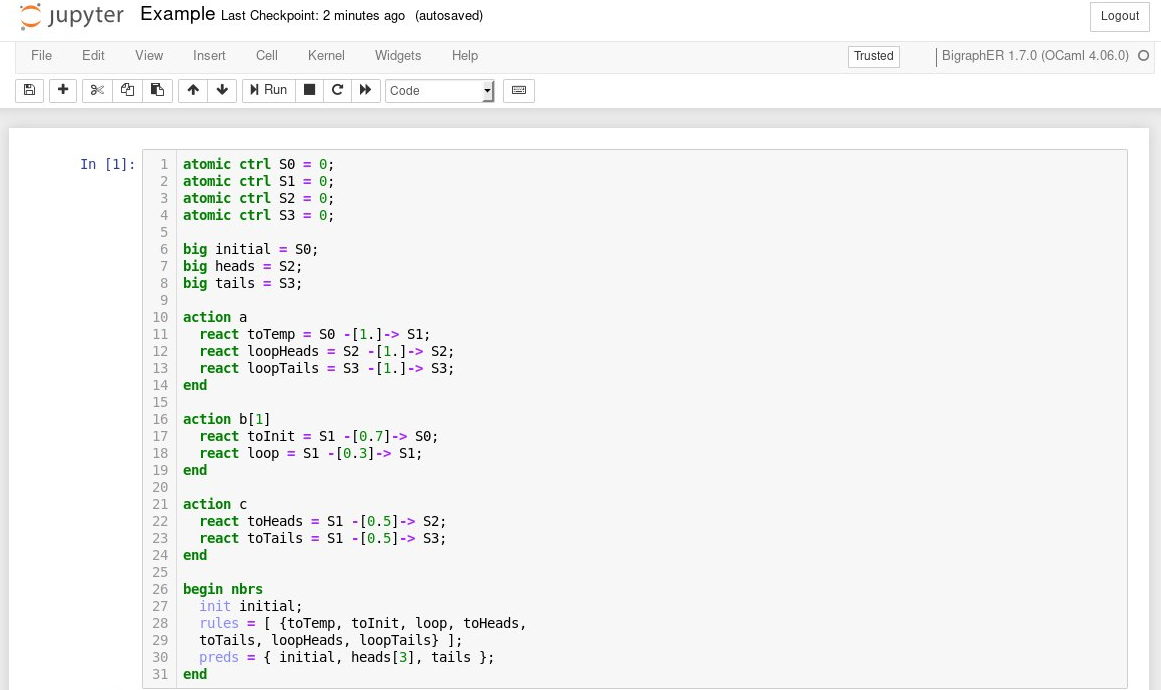
\includegraphics{images/interface.jpg}
  \caption{The BigraphER Jupyter interface with syntax highlighting.}
  \label{interface}
\end{figure}

\begin{figure}
  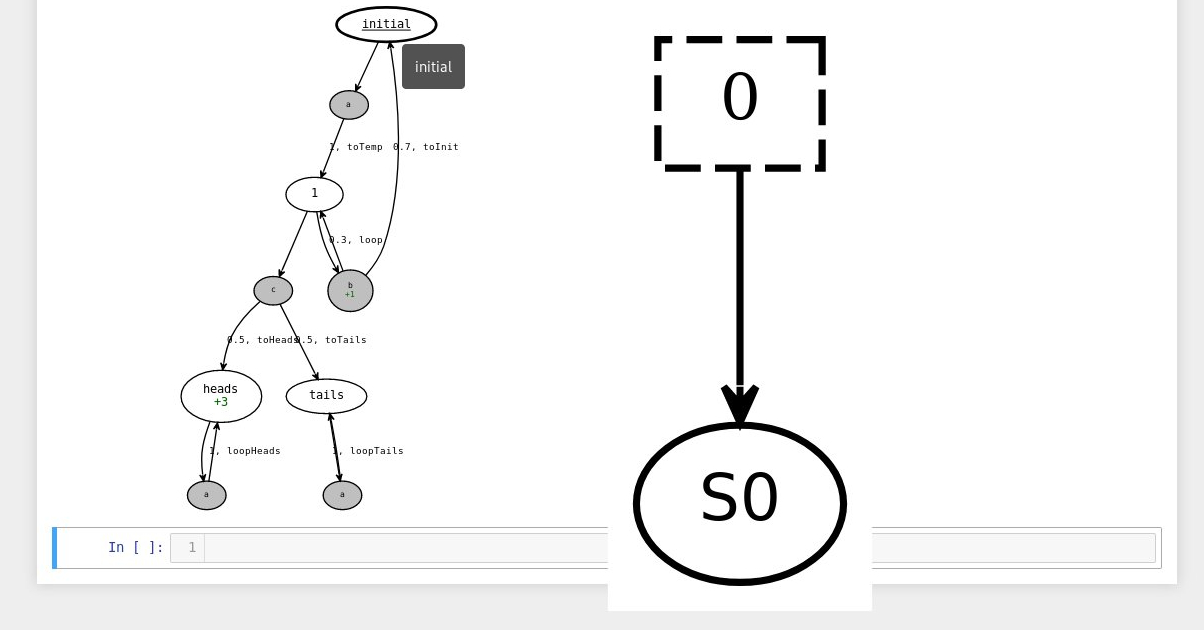
\includegraphics{images/transitions.jpg}
  \caption{...}
  \label{transitions}
\end{figure}

\begin{figure}
  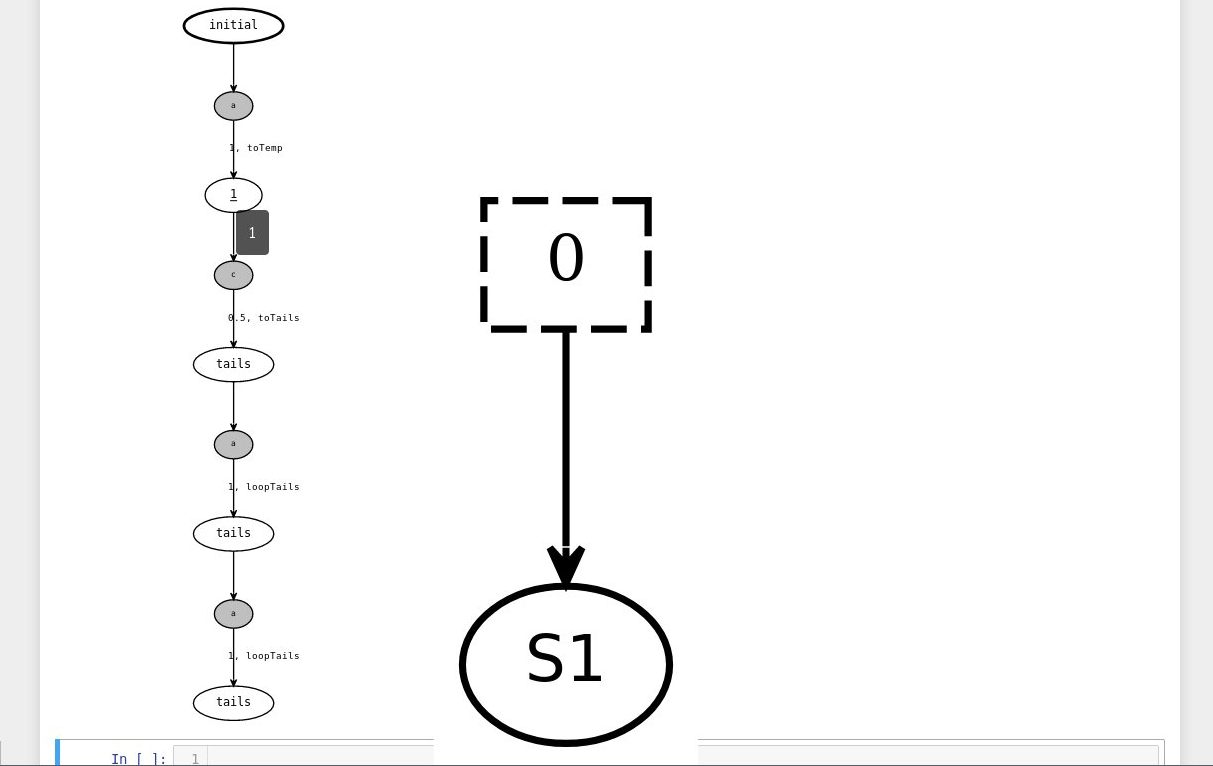
\includegraphics{images/simulation.jpg}
  \caption{...}
  \label{simulation}
\end{figure}

\begin{figure}
  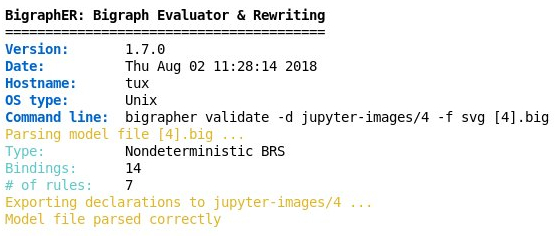
\includegraphics{images/output.jpg}
  \caption{...}
  \label{output}
\end{figure}

\section{Exporting to PRISM}

Transitions, state rewards, transition rewards

\section{Case study in autonomous agents}

\bibliographystyle{splncs04}
\bibliography{bibliography}
\end{document}
